\chapter{Instruction Tuning}
\label{ch:instruction-tuning}
\raggedbottom

In March 2023, a Stanford team fine-tuned LLaMA-7B on 52{,}000 instruction-response pairs generated by GPT-3.5. The reported training cost was under \$600, and the resulting model, Alpaca, behaved far more like an instruction-following assistant than the base checkpoint did~\cite{taori2023alpaca}. The same base model, without fine-tuning, was not a chat assistant. It could continue text, answer some questions, and complete patterns, but it did not reliably treat user requests as instructions. Same architecture, same starting checkpoint, same inference code. Different training data---52{,}000 examples---and visibly different behavior.

Part~II taught you to produce a pretrained language model: scale the architecture (Chapter~\ref{ch:what-changes}), distribute the computation (Chapter~\ref{ch:distributed-training}), allocate the budget (Chapter~\ref{ch:scaling-laws}), curate the data (Chapter~\ref{ch:data-engineering}), and evaluate the result (Chapter~\ref{ch:evaluation}). That model is a powerful text completer---and a terrible assistant. It does not follow instructions, does not decline harmful requests, and does not structure its outputs for human consumption. The gap between ``pretrained model'' and ``useful product'' is where most of modern LLM research now lives.

Part~III closes that gap. Its seven chapters cover the transformation from pretrained language model to instruction-following, preference-aligned, and (for reasoning models) capability-pushed system. This chapter---the first---teaches instruction tuning: the simplest and most impactful step in that transformation.

\paragraph{What this chapter covers.} Instruction tuning is not primarily about algorithmic novelty. The loss function is the same next-token cross-entropy from Chapter~\ref{ch:tokens-to-training}. What makes it powerful is \emph{what you train on}. This chapter teaches the mechanics and the data together, because in practice they are coupled: the format of the data determines the loss masking strategy, the data source determines the capability ceiling, and the data scale determines whether you need synthetic generation. Three questions organize the chapter:

\begin{enumerate}[nosep]
  \item \textbf{What are you training?} The mechanics of supervised fine-tuning---how the loss, the templates, and the training infrastructure change when you move from pretraining to instruction tuning (\S\ref{sec:finetuning-landscape}--\S\ref{sec:sft-infrastructure}).
  \item \textbf{Where does the data come from?} The source taxonomy, the synthetic generation pipeline, and the ongoing debate about quality versus quantity (\S\ref{sec:data-moat}--\S\ref{sec:distillation-data}).
  \item \textbf{What are the limits?} When SFT alone is enough, when it is not, and where InstructGPT fits in the modern landscape (\S\ref{sec:sft-limits}--\S\ref{sec:instructgpt-callout}).
\end{enumerate}

\paragraph{Running example.} You have a pretrained $\sim$900M model from Project~2. It predicts the next token competently but cannot follow a single instruction. By the end of this chapter, you will have a concrete recipe for turning it into an instruction-following model: what data to use, what format, what loss to compute, and what to expect. Project~3 makes this real.

\begin{figure}[ht]
\centering
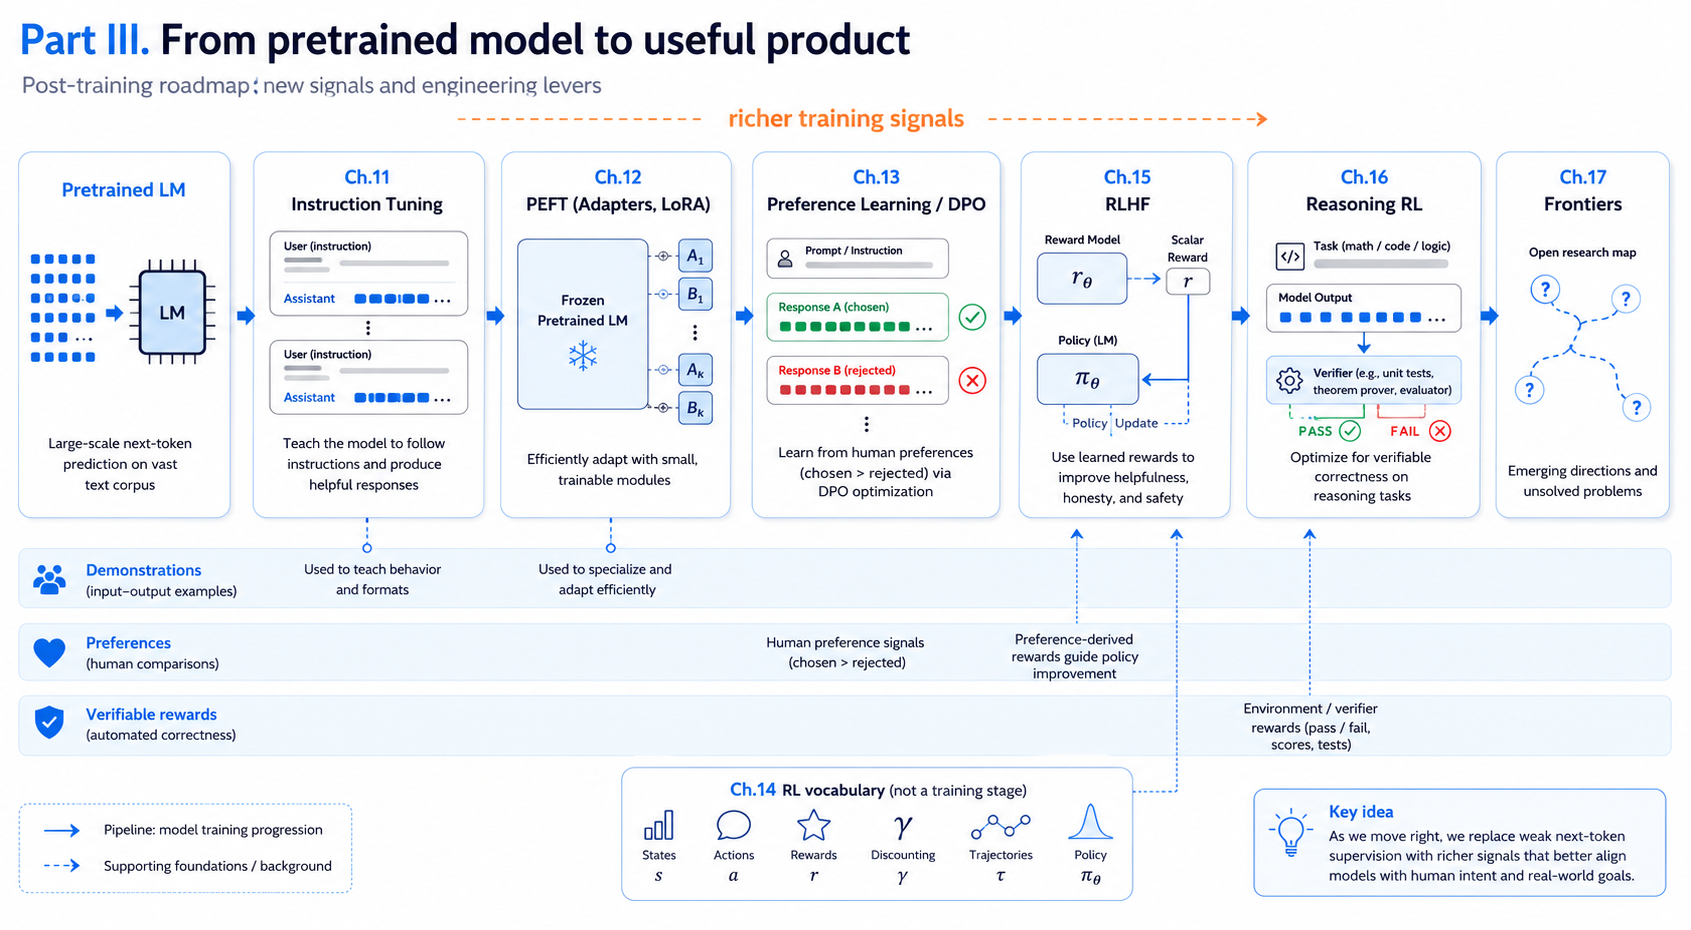
\includegraphics[width=0.95\textwidth]{figures/ch11/fig_part3_roadmap.png}
\caption{\textbf{Part~III roadmap.} The post-training pipeline transforms a pretrained language model into a useful product through progressively richer training signals. Instruction tuning (this chapter) uses demonstration data. PEFT (Chapter~\ref{ch:peft}) is the efficiency layer that can be applied to SFT, preference learning, or RL fine-tuning. Preference learning (Chapter~\ref{ch:preference-learning}) uses pairwise comparisons. RLHF (Chapter~\ref{ch:rlhf}) and reasoning RL (Chapter~\ref{ch:reasoning-rl}) use reward signals from humans, AI judges, or verifiers. Chapter~\ref{ch:rl-foundations} provides the RL foundations that Chapters~\ref{ch:rlhf}--\ref{ch:reasoning-rl} require. Chapter~\ref{ch:frontiers} surveys the open frontier.}
\label{fig:part3-roadmap}
\end{figure}


\subsection*{Learning Objectives}

After completing this chapter, you should be able to:

\begin{enumerate}
  \item Explain what fine-tuning means in the context of generative language models and distinguish instruction tuning from other fine-tuning paradigms.
  \item Write the masked cross-entropy loss used in SFT and explain why loss is computed only on assistant tokens.
  \item Parse a chat template (ChatML, Llama-3 format) and identify the role of special tokens, role markers, and EOS conventions.
  \item Describe sequence packing and attention masking for SFT, and explain why these engineering choices affect training efficiency and correctness.
  \item Classify instruction data sources into four categories (human-written, template-based, LLM-generated, distillation) and evaluate the trade-offs of each.
  \item Articulate the LIMA hypothesis, explain the subsequent reconciliation, and apply the quality-vs-quantity trade-off to a Project~3 data budget.
  \item Identify the capability ceiling of SFT and explain when preference learning or RL fine-tuning is needed.
\end{enumerate}


\subsection*{Notation}

\begin{center}
\begin{tabular}{ll}
\toprule
Symbol & Meaning \\
\midrule
$\theta$ & Model parameters \\
$\theta_0$ & Pretrained (base) model parameters \\
$x$ & Input tokens (instruction / user turns) \\
$y$ & Target tokens (response / assistant turns) \\
$\mathcal{L}_{\text{SFT}}$ & Supervised fine-tuning loss (masked cross-entropy) \\
$T$ & Sequence length \\
$m_t$ & Loss mask at position $t$ ($m_t = 1$ for assistant tokens, $0$ otherwise) \\
$\eta$ & Learning rate \\
\bottomrule
\end{tabular}
\end{center}


\subsection*{Timeline}

\begin{center}
\begin{tabularx}{\textwidth}{@{}lX@{}}
\toprule
\textbf{Year} & \textbf{Milestone} \\
\midrule
2021 & FLAN (Wei et al.): instruction tuning via NLP task templates at scale \\
2022 & InstructGPT (Ouyang et al.): three-stage recipe (SFT $\to$ RM $\to$ RLHF); SFT as Stage~1 \\
2022 & Self-Instruct (Wang et al.): LLM generates its own instruction data \\
2023 & Alpaca: 52K GPT-3.5-generated examples make LLaMA-7B behave like an instruction-following model \\
2023 & Vicuna: ShareGPT conversation data; user-collected demonstrations \\
2023 & LIMA (Zhou et al.): 1{,}000 curated examples challenge the assumption that more SFT data is always better \\
2023 & Tulu (Ivison et al.): systematic study of instruction data mixtures \\
2024+ & Llama-3-Instruct, Qwen-Instruct, Mistral-Instruct: curated SFT plus preference tuning becomes the open-model default \\
\bottomrule
\end{tabularx}
\end{center}


%======================================================================
% PART A: What Are You Training? (§11.1--§11.6)
%======================================================================

\section{Fine-Tuning: From Generalist to Specialist}
\label{sec:finetuning-landscape}

Pretraining produces a generalist: a model that has absorbed the statistical structure of a large text corpus and can predict the next token across many domains. Fine-tuning redirects that generalist toward a specific behavior. The mechanism is simple---continue training on a smaller, targeted dataset with a lower learning rate---but the consequences are large.

\paragraph{Why fine-tuning works.} The representations learned during pretraining are transferable. A model trained on trillions of tokens has learned syntax, world knowledge, reasoning patterns, and formatting conventions. Fine-tuning does not teach these from scratch. It steers the model's output distribution toward a new target: answer questions instead of continuing web text, follow instructions instead of generating plausible-sounding paragraphs, refuse harmful requests instead of complying.

\paragraph{The fine-tuning landscape.} Fine-tuning is not a single technique. It is a family of methods that differ in what data they use, what loss they optimize, and what behavior they produce. Part~III covers the major variants:

\begin{itemize}[nosep]
  \item \textbf{Instruction tuning} (this chapter): train on (instruction, response) pairs using the standard cross-entropy loss. The simplest and most widely used post-training method.
  \item \textbf{Preference fine-tuning} (Chapter~\ref{ch:preference-learning}): train on pairwise preference data using DPO or similar objectives. Aligns the model to human preferences without RL machinery.
  \item \textbf{RL fine-tuning} (Chapters~\ref{ch:rlhf}--\ref{ch:reasoning-rl}): optimize a reward signal using policy gradient methods. Required for RLHF alignment and reasoning capability.
\end{itemize}

Orthogonal to these three is \textbf{parameter-efficient fine-tuning} (PEFT; Chapter~\ref{ch:peft}): methods like LoRA and QLoRA that modify only a small subset of parameters, reducing memory cost by 4--16$\times$. PEFT specifies \emph{which parameters} get updated, not \emph{what objective} is being optimized---it can be applied to instruction tuning, preference learning, or RL fine-tuning alike.

Two related concepts that are \emph{not} Part~III's focus but worth distinguishing:

\begin{itemize}[nosep]
  \item \textbf{Continual pretraining}: extend pretraining on domain-specific data (e.g., medical text) to adapt the model's knowledge base. Same loss as pretraining, different data distribution.
  \item \textbf{Task-specific fine-tuning} (BERT era): add a classification head to a pretrained encoder and fine-tune on labeled examples. This is a different paradigm---the model architecture changes, and the task is classification, not generation. Modern LLM fine-tuning keeps the same architecture and the same generative loss; what changes is the data distribution.
\end{itemize}

\paragraph{Catastrophic forgetting.} Fine-tuning on a narrow dataset risks overwriting the broad capabilities learned during pretraining. A model fine-tuned exclusively on medical Q\&A may lose its ability to write code or discuss history. The standard mitigations are small learning rates (typically $10\times$--$100\times$ smaller than pretraining), short training durations (1--5 epochs), and diverse instruction data. Chapters~\ref{ch:preference-learning} and~\ref{ch:rlhf} will introduce KL constraints---a more principled solution that explicitly penalizes deviation from the pretrained distribution.

\paragraph{Chapter scope.} This chapter focuses on instruction tuning: the data is (instruction, response) pairs, the loss is cross-entropy on response tokens, and the goal is an instruction-following model. Everything else in the fine-tuning landscape is covered in subsequent chapters.

\begin{quickrecap}
\textbf{Quick Recap.}
\begin{itemize}[nosep,leftmargin=1.5em]
  \item Fine-tuning redirects pretrained representations toward a target behavior using smaller datasets and lower learning rates.
  \item Part~III covers three objective paradigms: instruction tuning, preference learning, and RL fine-tuning. PEFT is an orthogonal efficiency layer that can be applied to any of them.
  \item Catastrophic forgetting is the main risk; small LR, short training, and diverse data are the standard mitigations.
\end{itemize}
\textit{Next: what exactly changes when a pretrained model becomes an instruction-following model?}
\end{quickrecap}


%======================================================================
\section{From Completion to Instruction: What Changes}
\label{sec:completion-to-instruction}

A pretrained language model and an instruction-tuned model use the same architecture, the same tokenizer, and the same inference code. The difference is the conditional distribution they have learned to produce.

\paragraph{The base model.} Given a prefix, the pretrained model generates a plausible continuation. Prompt it with ``What is the capital of France?'' and it might generate:

\begin{verbatim}
  What is the capital of France?
  What is the capital of Germany?
  What is the capital of Italy?
\end{verbatim}

This is a perfectly reasonable web-text continuation---the model has learned that questions tend to appear in lists. It has not learned that questions are meant to be answered.

\paragraph{The instruction-tuned model.} The same architecture, fine-tuned on (instruction, response) pairs, generates:

\begin{verbatim}
  What is the capital of France?
  The capital of France is Paris.
\end{verbatim}

The model has learned a different conditional:
\[
P(\text{response} \mid \text{instruction})
\quad \text{instead of} \quad
P(\text{continuation} \mid \text{prefix}).
\]
The pretraining knowledge (``Paris is the capital of France'') was already there. Instruction tuning did not teach the fact---it taught the model to \emph{retrieve and format} the fact in response to a question.

\begin{figure}[t]
\centering
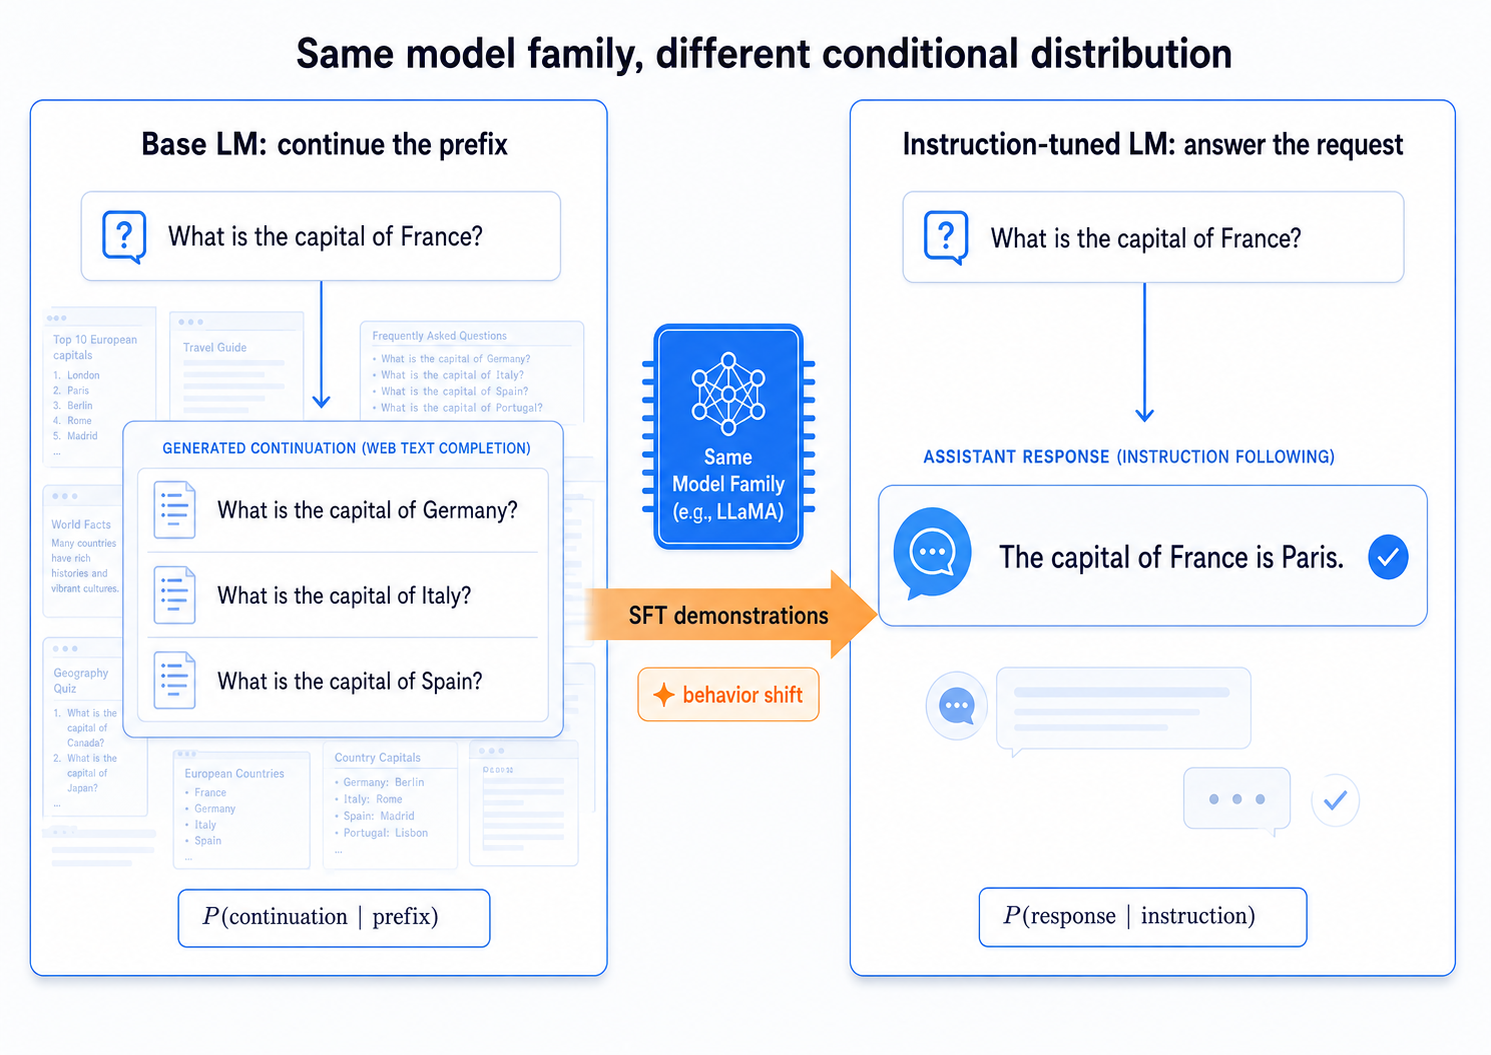
\includegraphics[width=0.92\textwidth]{figures/ch11/fig_completion_vs_instruction.png}
\caption{\textbf{Completion behavior versus instruction behavior.} A base model treats the prompt as a prefix to continue, while an instruction-tuned model treats it as a request to answer. The architecture and pretrained knowledge are the same; the post-training data changes which continuation the model considers appropriate.}
\label{fig:completion-vs-instruction}
\end{figure}

\paragraph{Distribution shift.} This is the core conceptual move: instruction tuning shifts the model's output distribution from ``what text typically follows this prefix on the internet'' to ``what text a helpful assistant would produce in response to this instruction.'' The shift is not about knowledge (that comes from pretraining) but about \emph{behavior}---how the model uses its knowledge.

\noindent\fbox{\parbox{\dimexpr\textwidth-2\fboxsep-2\fboxrule\relax}{%
\textbf{Pause and verify.}\quad Take any pretrained base model (e.g., Llama-3-8B base) and prompt it with: ``Summarize the following paragraph in one sentence: [paragraph].'' Now prompt Llama-3-8B-Instruct with the same input.

\smallskip
The base model may continue the text or generate another instruction. The instruct model is much more likely to produce a summary. \emph{Both models start from the same pretrained checkpoint. The difference is what they were trained to do after pretraining.}
}}

\begin{quickrecap}
\textbf{Quick Recap.}
\begin{itemize}[nosep,leftmargin=1.5em]
  \item Base models generate continuations; instruction-tuned models generate responses.
  \item The shift is behavioral, not knowledge-based: instruction tuning teaches the model to use its pretrained knowledge in response to directives.
  \item Same architecture, same tokenizer, different output distribution.
\end{itemize}
\textit{Next: the loss function that produces this behavioral shift---familiar math, new data.}
\end{quickrecap}


%======================================================================
\section{SFT Mechanics: Same Loss, Different Data}
\label{sec:sft-mechanics}

The supervised fine-tuning (SFT) loss is the same cross-entropy from Chapter~\ref{ch:tokens-to-training}---with one critical modification.

\paragraph{The standard causal LM loss.} During pretraining, every token in the sequence contributes to the loss:
\[
\mathcal{L}_{\text{pretrain}} = -\frac{1}{T}\sum_{t=1}^{T} \log p_\theta(x_t \mid x_{<t})
\]

During instruction tuning, the training sequence consists of an instruction (user input) followed by a response (assistant output). We only want the model to learn to \emph{produce} the response, not to memorize the instruction. So we mask the loss on instruction tokens:

\[
\boxed{\mathcal{L}_{\text{SFT}} = -\frac{1}{\sum_t m_t}\sum_{t=1}^{T} m_t \cdot \log p_\theta(x_t \mid x_{<t})}
\]

where $m_t = 1$ if token $t$ is an assistant (response) token, and $m_t = 0$ if it is a user (instruction) or system token. The denominator normalizes by the number of unmasked tokens.

\paragraph{Why mask the instruction?} Two reasons:

\begin{enumerate}[nosep]
  \item \textbf{Learning signal.} The model should learn to generate responses, not to parrot instructions. Including instruction tokens in the loss would reward the model for memorizing user queries---not a useful capability.
  \item \textbf{Distribution shift.} At inference time, the user provides the instruction. The model only generates the response. Training should match the inference distribution: learn from the tokens you will actually produce.
\end{enumerate}

\paragraph{What else changes.}

\begin{center}
\begin{tabularx}{\textwidth}{@{}lXX@{}}
\toprule
& \textbf{Pretraining} & \textbf{Instruction tuning (SFT)} \\
\midrule
Loss & All tokens & Response tokens only \\
Learning rate & $10^{-4}$--$10^{-3}$ & $10^{-5}$--$2\times10^{-5}$ \\
Dataset size & Billions--trillions of tokens & Thousands--millions of examples \\
Epochs & $<1$ (each token seen once) & 1--5 (each example seen multiple times) \\
Duration & Days--weeks & Hours--days \\
\bottomrule
\end{tabularx}
\end{center}

The learning rate is typically $10\times$--$100\times$ smaller than pretraining to avoid catastrophic forgetting. The dataset is $1{,}000\times$--$1{,}000{,}000\times$ smaller. Training duration is correspondingly shorter: a few hours to a few days, compared to weeks or months for pretraining.

\begin{tcolorbox}[colback=orange!5, colframe=orange!60, title=\textbf{For Project~3: SFT Hyperparameters}]
\begin{itemize}[nosep]
  \item \textbf{Learning rate:} $2 \times 10^{-5}$ with cosine decay to $2 \times 10^{-6}$. Your 900M model's pretraining LR was $\sim$$3 \times 10^{-4}$---SFT uses $\sim$$15\times$ less.
  \item \textbf{Epochs:} 3 over 50K instruction-response pairs.
  \item \textbf{Duration:} A few hours on a single GPU.
  \item \textbf{Batch size:} 32--64 effective examples (accumulate if needed).
\end{itemize}
\end{tcolorbox}

\begin{quickrecap}
\textbf{Quick Recap.}
\begin{itemize}[nosep,leftmargin=1.5em]
  \item SFT uses the same cross-entropy loss as pretraining, but masked to response tokens only.
  \item Learning rate is $10\times$--$100\times$ smaller; dataset is $1{,}000\times$+ smaller; training is hours, not weeks.
  \item The loss mask is the key technical difference: it tells the model ``imitate the assistant, not the user.''
\end{itemize}
\textit{Next: the data format that makes loss masking possible---chat templates.}
\end{quickrecap}


%======================================================================
\section{Chat Templates and Formatting}
\label{sec:chat-templates}

Loss masking requires knowing which tokens belong to which role. That information comes from the \textbf{chat template}---a structured format that marks role boundaries with delimiters, role tags, and sometimes dedicated special tokens.

\paragraph{ChatML (OpenAI).} One of the earliest standardized formats:

\begin{lstlisting}[language={},morekeywords={},deletekeywords={}]
<|im_start|>system
You are a helpful assistant.<|im_end|>
<|im_start|>user
What is the capital of France?<|im_end|>
<|im_start|>assistant
The capital of France is Paris.<|im_end|>
\end{lstlisting}

The markers \texttt{<|im\_start|>} and \texttt{<|im\_end|>} are not natural language. Depending on the tokenizer, they may be represented as dedicated special tokens or as reserved delimiter strings. Either way, the model learns to parse them as structural markers, not content.

\paragraph{Llama-3 chat format.}

\begin{lstlisting}[language={},morekeywords={},deletekeywords={}]
<|begin_of_text|><|start_header_id|>system<|end_header_id|>

You are a helpful assistant.<|eot_id|>
<|start_header_id|>user<|end_header_id|>

What is the capital of France?<|eot_id|>
<|start_header_id|>assistant<|end_header_id|>

The capital of France is Paris.<|eot_id|>
\end{lstlisting}

Different syntax, same function: mark role boundaries so the training pipeline knows where to apply the loss mask and the inference pipeline knows when to stop generating.

\begin{figure}[t]
\centering
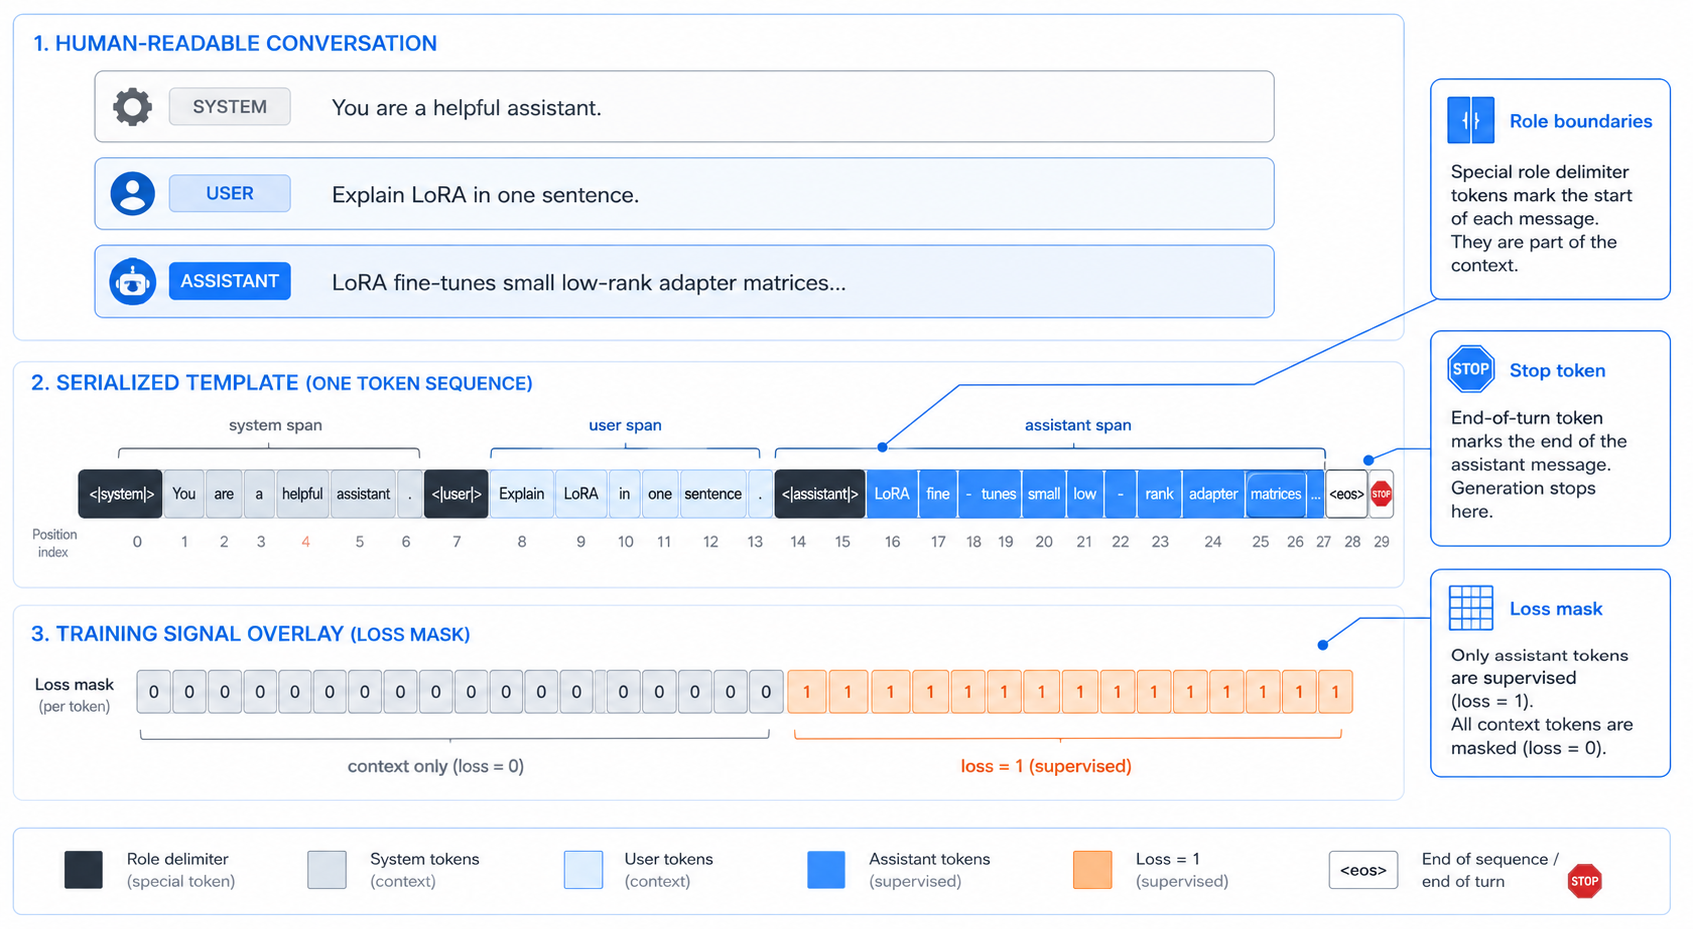
\includegraphics[width=0.92\textwidth]{figures/ch11/fig_chat_template_anatomy.png}
\caption{\textbf{Anatomy of a chat template.} System, user, and assistant spans are serialized into one token sequence with role delimiters. The same structure controls both generation boundaries and loss masking: user tokens are context, assistant tokens are behavior to imitate.}
\label{fig:chat-template-anatomy}
\end{figure}

\paragraph{Why format matters.} The chat template is not cosmetic. It determines:

\begin{itemize}[nosep]
  \item \textbf{Loss masking boundaries}: the training code uses template tokens to compute $m_t$. A wrong template means training on user tokens or masking assistant tokens---both silently degrade the model.
  \item \textbf{EOS behavior}: the model must learn to stop generating at the end of its turn. The \texttt{<|im\_end|>} or \texttt{<|eot\_id|>} token serves as the stop signal. If training data is inconsistent about where this token appears, the model will either generate indefinitely or stop mid-sentence.
  \item \textbf{System prompt}: the system message sets behavioral context (``You are a helpful assistant'' vs ``You are a medical expert''). The model conditions on this at inference time, so it must appear consistently in training data.
\end{itemize}

\begin{tcolorbox}[colback=blue!3, colframe=blue!40, title={\small Template Mismatch Is a Silent Failure}]
A common SFT bug: the training data uses one chat template, but the inference code applies a different one. The model was trained to respond after \texttt{<|im\_end|>}\texttt{<|im\_start|>assistant}, but at inference time it sees \texttt{<|eot\_id|>}\texttt{<|start\_header\_id|>assistant}. The tokens are different; the model's learned conditional does not activate. The result is incoherent or off-topic generation---and because the model still produces grammatical text, the bug is easy to miss. \textbf{Always verify that training and inference templates are identical.}
\end{tcolorbox}

\begin{quickrecap}
\textbf{Quick Recap.}
\begin{itemize}[nosep,leftmargin=1.5em]
  \item Chat templates (ChatML, Llama-3 format) use special tokens to mark role boundaries.
  \item The template determines loss masking, EOS behavior, and system prompt conditioning.
  \item Template mismatch between training and inference is a common, silent failure mode.
\end{itemize}
\textit{Next: what happens when training data contains multi-turn conversations, not just single exchanges?}
\end{quickrecap}


%======================================================================
\section{Multi-Turn Conversation as Training Data}
\label{sec:multi-turn}

Real assistant interactions are multi-turn: a user asks a question, the assistant responds, the user follows up, and the conversation continues. Training on multi-turn data teaches the model to maintain context, reference earlier turns, and handle follow-up questions.

\paragraph{Concatenation.} A multi-turn conversation is concatenated into a single training sequence:

\begin{center}
\small
\texttt{[system] [user\_1] [assistant\_1] [user\_2] [assistant\_2] ... [user\_n] [assistant\_n]}
\end{center}

The loss mask is applied to all assistant turns: $m_t = 1$ for tokens in any \texttt{assistant\_k} segment, $m_t = 0$ for system and user tokens. The model learns to produce each assistant turn conditioned on the entire conversation history up to that point.

\paragraph{Training implications.}

\begin{itemize}[nosep]
  \item \textbf{Context length.} Multi-turn conversations can be long. A 5-turn conversation with 200 tokens per turn is 1{,}000 tokens---within context limits. A 20-turn conversation with detailed responses can exceed 8K tokens. If your model's context window is 2K (common for smaller models), you must truncate or skip long conversations.
  \item \textbf{Turn quality.} Not all turns in a conversation are equally useful. Early turns may be greetings; later turns may contain the substantive interaction. Some practitioners weight later turns more heavily in the loss, though this is not standard.
  \item \textbf{Single-turn vs multi-turn mix.} A training set that is entirely multi-turn may underperform on single-turn instructions (the model learns to expect follow-ups). A mix of single-turn and multi-turn data is standard practice.
\end{itemize}

\begin{tcolorbox}[colback=orange!5, colframe=orange!60, title=\textbf{For Project~3: Multi-Turn Data Budget}]
\begin{itemize}[nosep]
  \item At 900M parameters with a 2K context window, multi-turn training is feasible but limited to short conversations (3--5 turns).
  \item Prioritize single-turn instruction-response pairs for the bulk of training ($\sim$80--90\%).
  \item Reserve 10--20\% of the data budget for multi-turn conversations to teach conversational coherence.
\end{itemize}
\end{tcolorbox}

\begin{quickrecap}
\textbf{Quick Recap.}
\begin{itemize}[nosep,leftmargin=1.5em]
  \item Multi-turn conversations are concatenated into single sequences; loss mask covers all assistant turns.
  \item Context length limits how many turns fit in one training example.
  \item A mix of single-turn and multi-turn data is standard; single-turn alone produces a model that struggles with follow-ups.
\end{itemize}
\textit{Next: the engineering tricks that make SFT training efficient---packing, masking, and loss computation.}
\end{quickrecap}


%======================================================================
\section{Training Infrastructure: Packing, Masking, and Loss}
\label{sec:sft-infrastructure}

Instruction-tuning datasets have highly variable sequence lengths: some examples are 50 tokens, others are 2{,}000. Na\"ive padding wastes compute. This section covers the engineering that makes SFT efficient.

\subsection{Sequence Packing}

Instead of padding every example to the maximum sequence length, pack multiple short examples into a single training sequence:

\begin{center}
\small
\texttt{[example\_1] [example\_2] [example\_3] [PAD...]}
\end{center}

A 2{,}048-token sequence might contain three 500-token examples and 548 tokens of padding---far less waste than three separate sequences each padded to 2{,}048. Packing can improve training throughput by $2\times$--$4\times$ on datasets with high length variance.

\subsection{Attention Masking Across Packed Examples}

Packing introduces a subtle correctness issue: without modification, the attention mechanism allows example~2 to attend to example~1's tokens. The examples are unrelated, so this creates cross-example leakage. The strict fix is a \textbf{block-diagonal attention mask}: each packed example can only attend to its own tokens. In practice, this means maintaining a ``document ID'' for each token and masking cross-document attention. Some high-throughput pipelines instead separate packed examples with EOS tokens and tolerate weak leakage, because the simpler causal mask is faster and easier to implement. For Project~3, the important point is to know which choice your trainer makes; do not assume that ``packing'' automatically implies document-isolated attention.

\begin{figure}[ht]
\centering
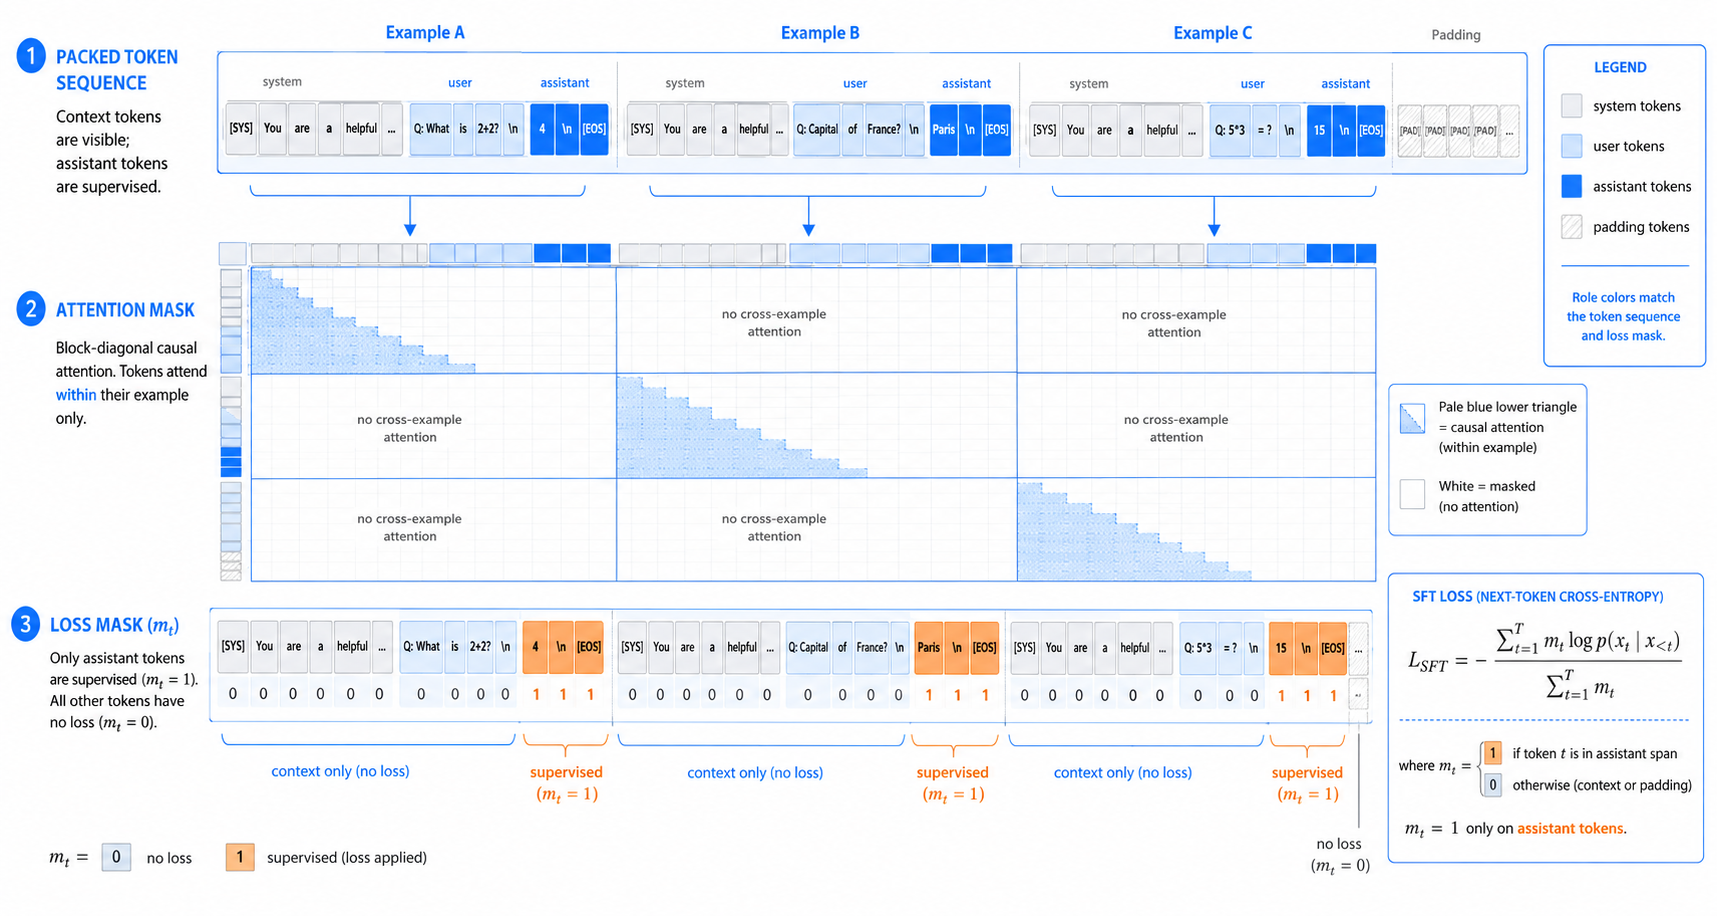
\includegraphics[width=0.9\textwidth]{figures/ch11/fig_packing_masking.png}
\caption{\textbf{Sequence packing with attention masking and loss masking.} Three instruction-response examples are packed into one training sequence. The attention mask is block-diagonal---each example attends only to itself. The loss mask selects only assistant tokens (shaded). User and system tokens contribute to attention context but not to the gradient.}
\label{fig:packing-masking}
\end{figure}

\subsection{Loss Masking in Practice}

The loss computation combines two masks:

\begin{enumerate}[nosep]
  \item \textbf{Role mask}: $m_t = 1$ for assistant tokens, $m_t = 0$ for user/system tokens (from \S\ref{sec:sft-mechanics}).
  \item \textbf{Padding mask}: $m_t = 0$ for padding tokens.
\end{enumerate}

The final mask is the logical AND: a token contributes to the loss only if it is both an assistant token and not padding. This two-layer masking is implemented once in the data pipeline and applied at every training step.

\noindent\fbox{\parbox{\dimexpr\textwidth-2\fboxsep-2\fboxrule\relax}{%
\textbf{Pause and verify.}\quad You pack two examples into one sequence. Example~A is a 300-token instruction with a 200-token response. Example~B is a 100-token instruction with a 400-token response. The sequence length is 2{,}048.

\smallskip
How many tokens are padding? How many tokens contribute to the loss?

\smallskip
\emph{Answer:} Total content: $300 + 200 + 100 + 400 = 1{,}000$ tokens. Padding: $2{,}048 - 1{,}000 = 1{,}048$ tokens. Loss tokens: $200 + 400 = 600$ (only assistant responses). Only 29\% of tokens in this sequence contribute to the gradient---this is normal for SFT.
}}

\paragraph{Callback to distributed training.} If you are fine-tuning on multiple GPUs (Chapter~\ref{ch:distributed-training}), the same data-parallel and model-parallel strategies apply. However, SFT datasets are small enough that a single GPU often suffices: 50K examples at 500 tokens each is 25M tokens---a few hours on one H100. For Project~3, single-GPU training is likely sufficient.

\begin{quickrecap}
\textbf{Quick Recap.}
\begin{itemize}[nosep,leftmargin=1.5em]
  \item Sequence packing fills training sequences with multiple examples, improving throughput $2\times$--$4\times$.
  \item Packed examples need an explicit policy for cross-example attention: block-diagonal masks prevent leakage; EOS-only packing is simpler but less clean.
  \item Loss masking combines role masks (assistant only) and padding masks; typically $<$50\% of tokens in a packed sequence contribute to the gradient.
\end{itemize}
\textit{Next: the mechanics are settled. Now the harder question: where does the instruction data come from?}
\end{quickrecap}


%======================================================================
% PART B: Where Does the Data Come From? (§11.7--§11.11)
%======================================================================

\section{Why Data Is the Moat}
\label{sec:data-moat}

Chapter~\ref{ch:data-engineering} established that pretraining data is a hidden scaling axis---data quality can rival the effect of doubling compute. The same principle applies to instruction tuning, but even more sharply.

\paragraph{The modern post-training thesis.} The SFT algorithm is shared: everyone uses masked cross-entropy. The optimizer is shared: AdamW with cosine decay. The architecture is shared: standard Transformer. \textbf{What differentiates instruction-tuned models is their data.} Llama-3-Instruct vs Qwen-2-Instruct vs Mistral-Instruct differ primarily in the instruction data they trained on---its quality, coverage, format, and composition.

This is not just a slogan. The Tulu study~\cite{ivison2023tulu} systematically varied instruction data mixtures while holding the model and training recipe fixed. The result: data composition explained a large part of downstream performance variation. Better data produced better models; changing the algorithm while leaving the data unchanged often produced smaller gains.

\paragraph{What ``data quality'' means for SFT.} In pretraining (Chapter~\ref{ch:data-engineering}), quality meant filtering out noise, deduplication, and domain coverage. In instruction tuning, quality has additional dimensions:

\begin{itemize}[nosep]
  \item \textbf{Instruction clarity}: unambiguous, well-formed instructions that specify the expected behavior.
  \item \textbf{Response quality}: responses that are correct, helpful, well-structured, and appropriately detailed.
  \item \textbf{Diversity}: coverage across task types (Q\&A, summarization, coding, math, creative writing, multi-turn dialogue).
  \item \textbf{Format consistency}: consistent use of chat template, role markers, and response style.
\end{itemize}

A dataset with 10{,}000 high-quality, diverse examples can outperform one with 100{,}000 mediocre examples. We will examine this claim---and its limits---in \S\ref{sec:lima-debate}.

\begin{quickrecap}
\textbf{Quick Recap.}
\begin{itemize}[nosep,leftmargin=1.5em]
  \item The SFT algorithm is commoditized; data is the differentiator.
  \item Instruction data quality has four dimensions: instruction clarity, response quality, diversity, and format consistency.
  \item The Tulu studies show that data composition explains a large part of downstream performance variation.
\end{itemize}
\textit{Next: a taxonomy of where instruction data comes from---four sources, four trade-off profiles.}
\end{quickrecap}


%======================================================================
\section{Source Taxonomy}
\label{sec:source-taxonomy}

Instruction data comes from four broad sources, each with a different quality--cost--scale profile:

\begin{center}
\begin{tabularx}{\textwidth}{@{}p{3cm}XXp{2.8cm}@{}}
\toprule
\textbf{Source} & \textbf{Strengths} & \textbf{Weaknesses} & \textbf{Typical scale} \\
\midrule
Human-written demonstrations & Highest quality; natural diversity; captures real user intent & Expensive (\$5--\$50/example); slow; annotator fatigue & 1K--50K \\
Template-based (FLAN) & Massive scale; broad task coverage; deterministic & Formulaic; narrow response style; limited to existing NLP tasks & 100K--10M \\
LLM-generated (Self-Instruct) & Cheap; fast; scalable & Quality ceiling set by teacher model; repetitive; potential legal issues & 50K--1M \\
Distillation from frontier models & Highest response quality at scale & Model-dependent; legal ambiguity; may ``collapse'' diversity & 50K--500K \\
\bottomrule
\end{tabularx}
\end{center}

\begin{figure}[ht]
\centering
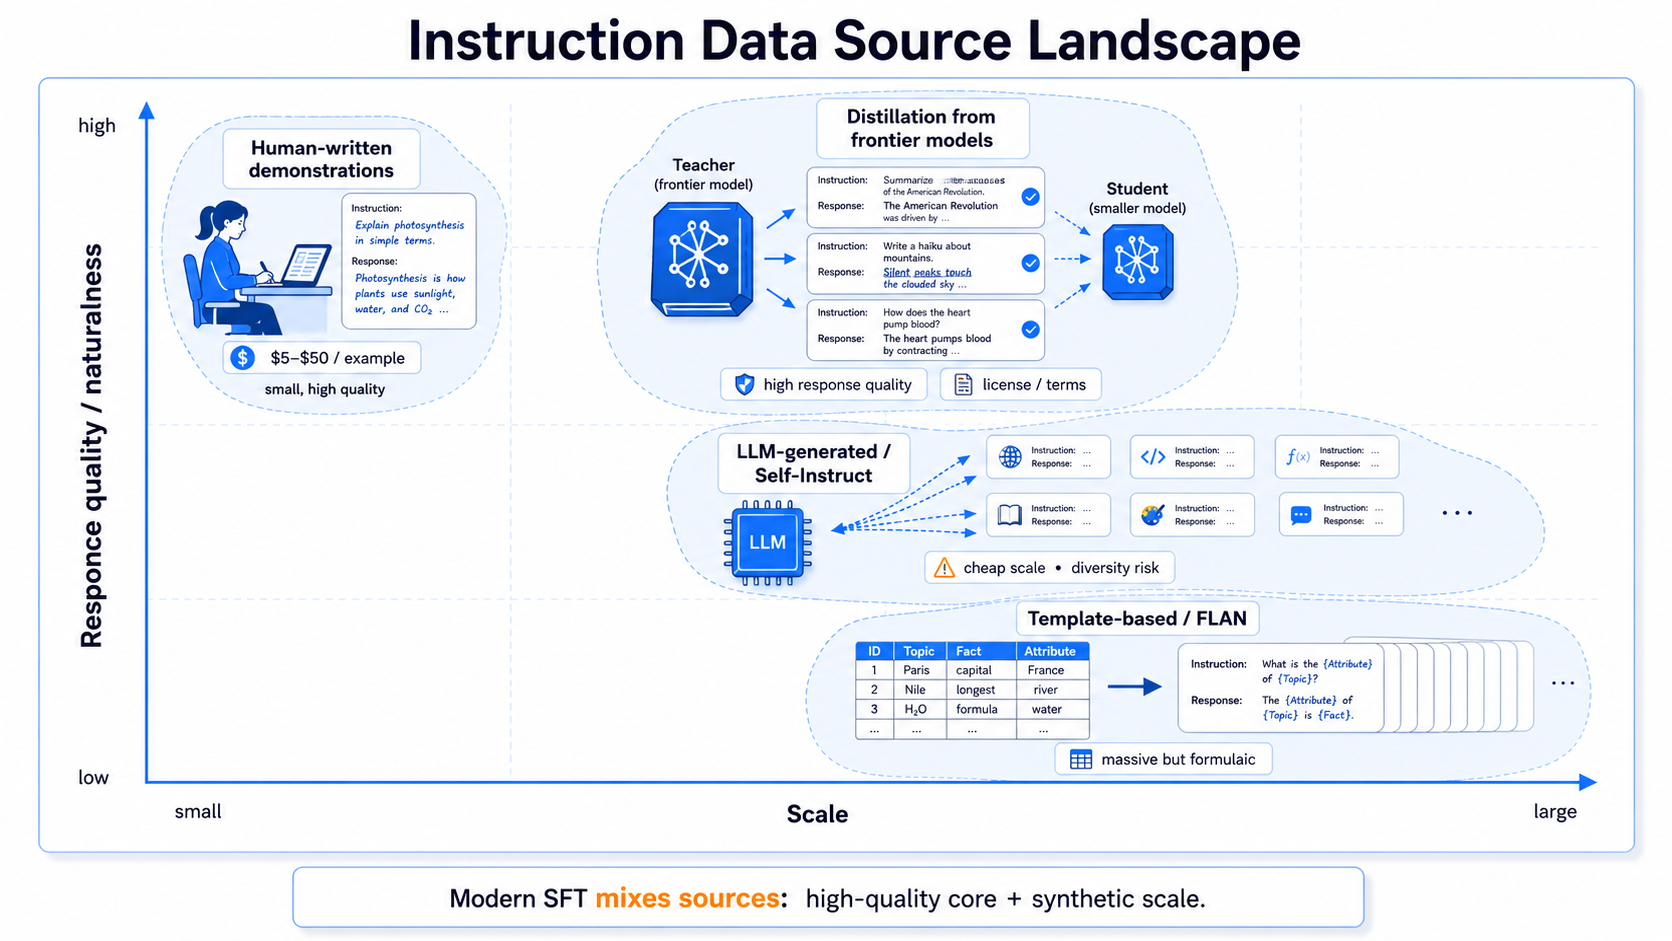
\includegraphics[width=0.9\textwidth]{figures/ch11/fig_source_taxonomy.png}
\caption{\textbf{Instruction data source landscape.} The four source categories occupy different regions of the quality--scale trade-off space. Human-written data is highest quality but smallest scale. Template-based data is massive but formulaic. LLM-generated and distillation data fill the middle ground. Modern practice combines multiple sources.}
\label{fig:source-taxonomy}
\end{figure}

\paragraph{Human-written demonstrations.} The gold standard: a human annotator reads an instruction and writes a response. InstructGPT's SFT stage used $\sim$13K human-written demonstrations. Anthropic's HH dataset includes human-written helpful and harmless responses. The quality is high, but the cost (\$5--\$50 per example, depending on task complexity and annotator expertise) limits scale.

\paragraph{Template-based (FLAN paradigm).} FLAN~\cite{wei2022flan} converted existing NLP datasets (sentiment analysis, translation, QA, summarization) into instruction format using hand-written templates. Example: the SST-2 sentiment dataset becomes ``Classify the sentiment of the following review as positive or negative: [review]. Sentiment:'' This produces millions of instruction-response pairs at zero marginal cost, but the responses are formulaic and the task distribution is limited to what existing NLP benchmarks cover.

\paragraph{LLM-generated (Self-Instruct).} The model generates its own training data. Self-Instruct~\cite{wang2023selfinstruct} prompted GPT-3 to generate instructions and then generated responses to those instructions; Alpaca later adapted this recipe with GPT-3.5 to produce 52K examples for LLaMA fine-tuning. This approach is cheap, fast, and scalable---but the quality is bounded by the teacher model, and the diversity can collapse (the model generates variations of the same instruction types).

\paragraph{Distillation from frontier models.} Similar to LLM-generated, but with a deliberate quality focus: use a frontier model (GPT-4, Claude, Gemini) to generate responses to curated instructions. The Phi~\cite{gunasekar2023phi} family used this approach to generate ``textbook quality'' synthetic data. The responses can be more consistent and detailed than ordinary crowd-written data, but training on another model's outputs raises licensing, terms-of-service, and ecosystem-diversity concerns.

\begin{quickrecap}
\textbf{Quick Recap.}
\begin{itemize}[nosep,leftmargin=1.5em]
  \item Four sources: human-written, template-based, LLM-generated, distillation. Each occupies a different quality--cost--scale niche.
  \item Modern practice mixes sources: high-quality human core + scaled synthetic expansion.
  \item The legal status of distillation data is an active area of concern.
\end{itemize}
\textit{Next: the Self-Instruct pipeline in detail---the technique that democratized instruction tuning.}
\end{quickrecap}


%======================================================================
\section{Self-Instruct Lineage and Synthetic Generation}
\label{sec:self-instruct}

Self-Instruct~\cite{wang2023selfinstruct} showed that a pretrained language model can generate its own instruction-tuning data. The pipeline is straightforward:

\begin{enumerate}[nosep]
  \item Start with a small seed set of human-written instructions ($\sim$175 in the original paper).
  \item Prompt the LLM to generate new instructions inspired by the seed set.
  \item For each generated instruction, prompt the LLM to generate a response.
  \item Filter: remove duplicates, low-quality examples, and examples too similar to the seed set.
  \item Repeat, using the growing dataset as expanded context.
\end{enumerate}

\begin{figure}[ht]
\centering
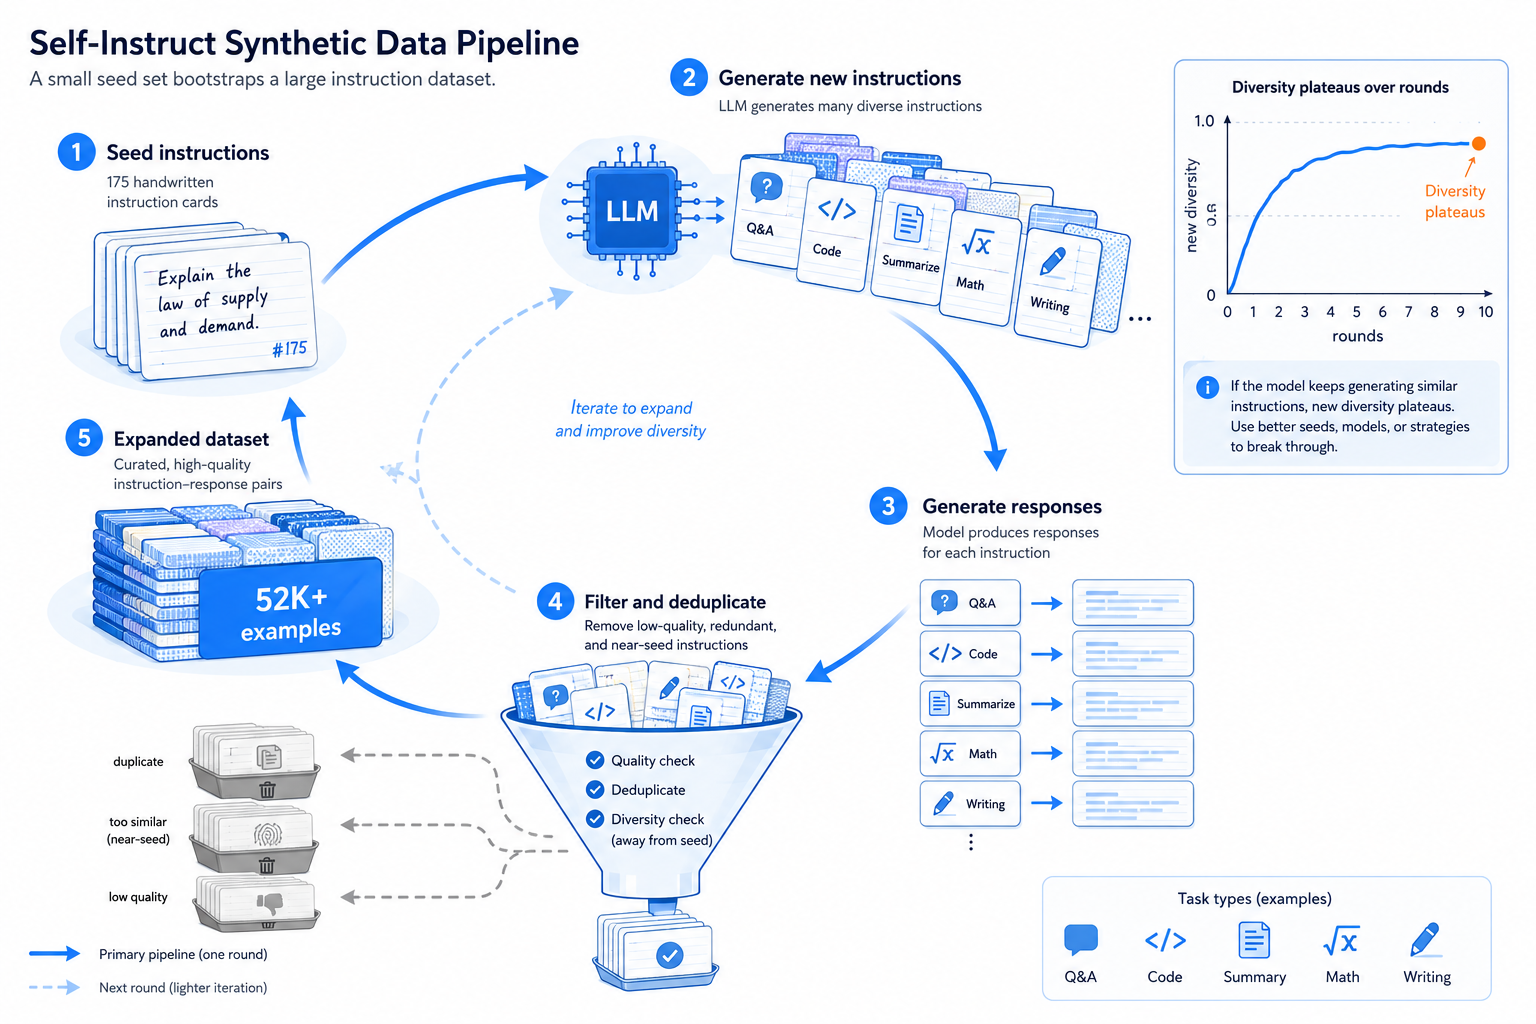
\includegraphics[width=0.9\textwidth]{figures/ch11/fig_self_instruct.png}
\caption{\textbf{The Self-Instruct pipeline.} A small seed set of human-written instructions bootstraps a larger synthetic dataset through iterative LLM generation and filtering. Each cycle expands the instruction space, though diversity tends to plateau after several rounds.}
\label{fig:self-instruct}
\end{figure}

\subsection{The Alpaca Moment}

Stanford's Alpaca project~\cite{taori2023alpaca} applied a Self-Instruct-style recipe using GPT-3.5 as the teacher, generating 52K examples at a reported cost of about \$500. Fine-tuning LLaMA-7B on this data produced a model whose behavior was surprisingly assistant-like for the cost and model size, though it was not a drop-in replacement for GPT-3.5. The result demonstrated that instruction tuning was no longer a frontier-lab exclusive.

\subsection{Vicuna and User-Generated Data}

Vicuna~\cite{chiang2023vicuna} took a different approach: instead of synthetic generation, it fine-tuned on $\sim$70K conversations from ShareGPT, a platform where users shared their ChatGPT interactions. The responses were generated by GPT-3.5/4, but the instructions came from real users---capturing genuine use patterns (debugging code, writing emails, brainstorming) that synthetic pipelines often miss.

\subsection{Tulu: Systematic Study of Mixtures}

The Tulu project~\cite{ivison2023tulu} systematically compared instruction data sources. Key findings:

\begin{itemize}[nosep]
  \item No single source was best across all benchmarks.
  \item Mixing sources (FLAN + ShareGPT + code instructions + safety data) consistently outperformed any single source.
  \item Quality filtering within each source mattered more than increasing scale.
\end{itemize}

\subsection{The Quality Ceiling}

Synthetic generation has a fundamental limit: the generated data cannot exceed the teacher model's capability. Alpaca's responses, generated by GPT-3.5, inherit GPT-3.5's limitations---factual errors, reasoning failures, and stylistic patterns. Fine-tuning a smaller model on these responses transfers both the capabilities and the limitations. This ceiling can be partially raised by generating from a stronger teacher (GPT-4 instead of GPT-3.5), but the underlying constraint remains.

\begin{quickrecap}
\textbf{Quick Recap.}
\begin{itemize}[nosep,leftmargin=1.5em]
  \item Self-Instruct bootstraps instruction data from a small seed set via iterative LLM generation.
  \item Alpaca demonstrated that instruction tuning is accessible: 52K synthetic examples, under \$600.
  \item Tulu showed that mixing sources is often stronger than relying on any single source; quality filtering can matter as much as scale.
  \item Synthetic data quality is capped by the teacher model's capability.
\end{itemize}
\textit{Next: can you skip scale entirely and just curate a few perfect examples?}
\end{quickrecap}


%======================================================================
\section{The LIMA Debate}
\label{sec:lima-debate}

In May 2023, Zhou et al.\ published LIMA~\cite{zhou2023lima}, a provocatively simple result: fine-tuning LLaMA-65B on just 1{,}000 carefully curated instruction-response pairs produced a model that remained competitive in a nontrivial fraction of blind comparisons against much larger assistants. The paper's thesis, crystallized in its title (``Less Is More for Alignment''), was that alignment is primarily about surfacing pretrained capabilities, not teaching new ones---and therefore a small, high-quality dataset can go surprisingly far.

\begin{tcolorbox}[colback=blue!3, colframe=blue!40, title={\small The LIMA Hypothesis}]
``A model's knowledge and capabilities are learnt almost entirely during pretraining, while alignment teaches it which subdistribution of formats should be used when interacting with users.''~\cite{zhou2023lima}

\smallskip
If this is true, then instruction tuning is not about teaching the model \emph{what} to do---it already knows---but about teaching it \emph{how} to present what it knows. A small number of high-quality demonstrations suffices to redirect the output distribution.
\end{tcolorbox}

\begin{figure}[t]
\centering
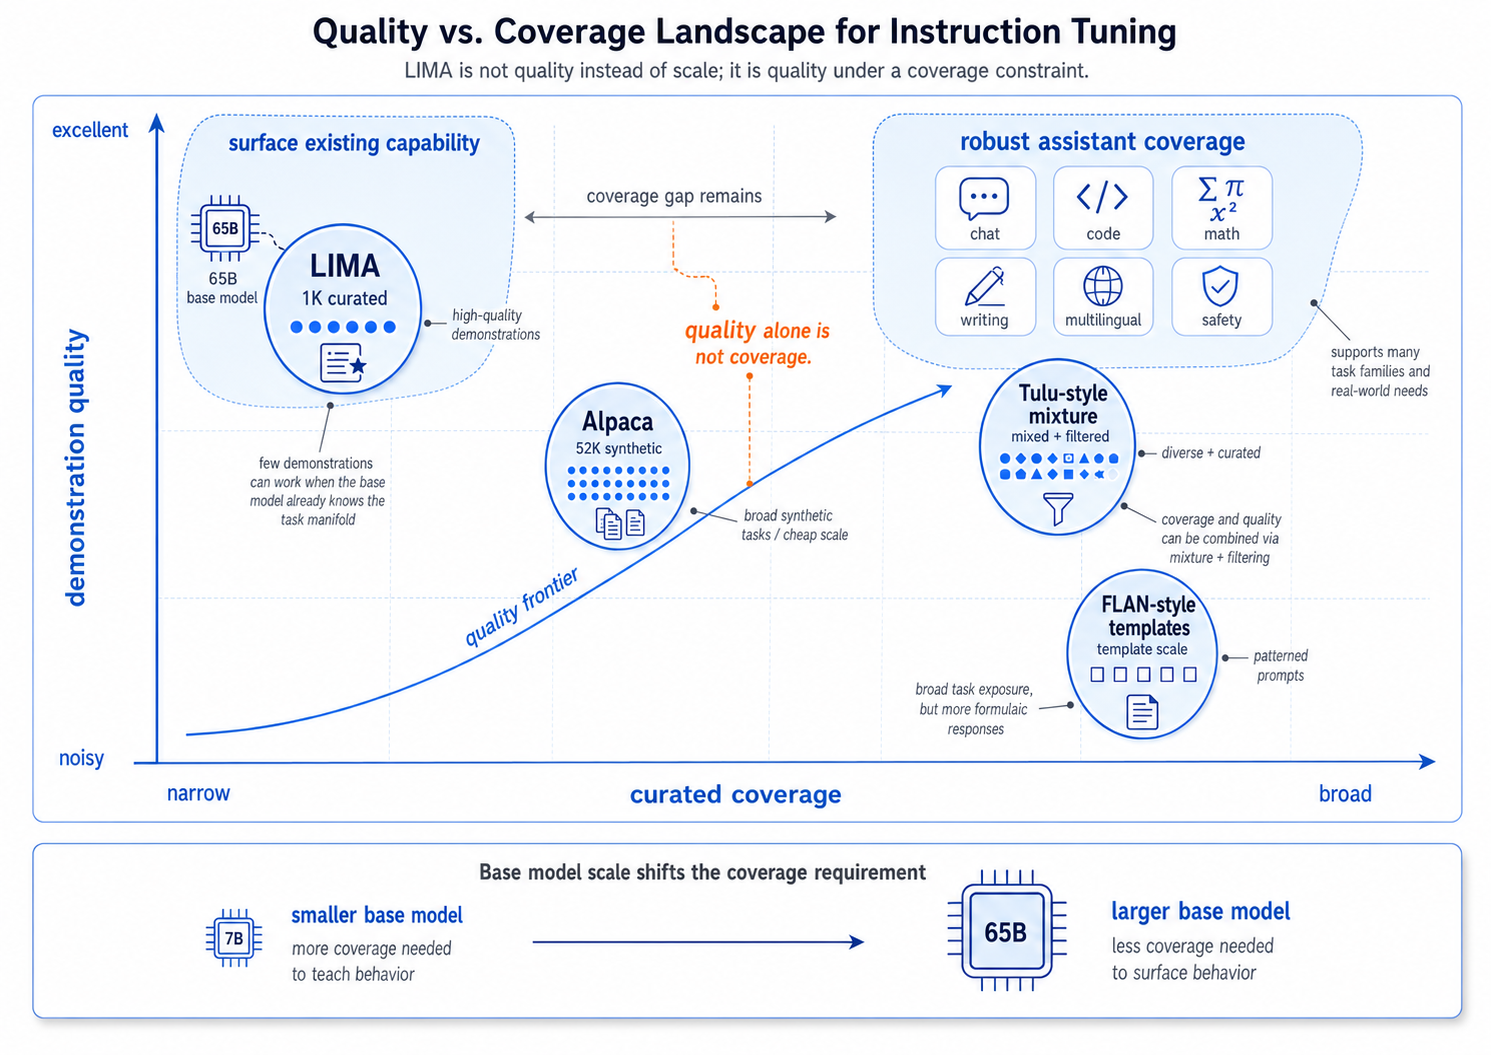
\includegraphics[width=0.9\textwidth]{figures/ch11/fig_lima_quality_coverage.png}
\caption{\textbf{The LIMA quality--coverage trade-off.} Small, carefully curated datasets can strongly redirect capable base models, but coverage becomes the limiting factor as task diversity grows. The practical question is not quality versus scale; it is how much curated coverage the model needs at its capability level.}
\label{fig:lima-quality-coverage}
\end{figure}

\paragraph{The subsequent reconciliation.} LIMA was influential but the full picture is more nuanced:

\begin{itemize}[nosep]
  \item \textbf{Quality dominates at small scale.} For $<$10K examples, curation quality is often the primary driver of performance. LIMA's result is real enough to take seriously.
  \item \textbf{Scale matters for coverage.} 1{,}000 examples cannot cover the full instruction space: multi-turn dialogue, code generation, mathematical reasoning, creative writing, multilingual tasks. A model trained on 1K examples is brittle on task types not represented in the training set. Later instruction-mixture studies showed continued gains from broader, carefully filtered mixtures.
  \item \textbf{The 65B caveat.} LIMA used a 65B-parameter base model with enormous pretrained capability. The ``surfacing'' thesis---SFT just redirects existing knowledge---is more plausible at 65B than at 7B, where the base model may not have the capabilities to surface.
  \item \textbf{Practical consensus (2024+).} Most modern instruction-tuned models use 50K--500K examples. The data is curated for quality (not scraped indiscriminately), but scale provides coverage that curation alone cannot.
\end{itemize}

\begin{tcolorbox}[colback=orange!5, colframe=orange!60, title=\textbf{For Project~3: The LIMA Lesson at 900M Scale}]
\begin{itemize}[nosep]
  \item At 900M parameters, your base model has limited pretrained capability. The LIMA ``surfacing'' thesis applies less directly---you are partially teaching capabilities, not just redirecting them.
  \item Use at least 20K--50K instruction examples, with emphasis on quality (correct responses, diverse tasks) rather than raw scale.
  \item If you must choose between 5K excellent but narrow examples and 50K reasonably filtered examples, choose the 50K---your model needs the coverage more than a 65B model does. Do not choose 50K low-quality examples.
\end{itemize}
\end{tcolorbox}

\begin{quickrecap}
\textbf{Quick Recap.}
\begin{itemize}[nosep,leftmargin=1.5em]
  \item LIMA showed that 1K curated examples can go surprisingly far---especially at large model scale and on covered task types.
  \item The reconciliation: quality dominates at small scale, but scale provides coverage. A common practical range is 50K--500K curated examples.
  \item At 900M parameters, scale matters more than at 65B---the model has less pretrained capability to surface.
\end{itemize}
\textit{Next: the most powerful and most controversial data source---distillation from frontier models.}
\end{quickrecap}


%======================================================================
\section{Distillation-Based Instruction Data}
\label{sec:distillation-data}

Distillation---using a stronger model's outputs as training data for a smaller model---is one of the most effective ways to produce high-quality instruction data at scale. It is also one of the most legally and ethically contested.

\paragraph{The approach.} Collect a set of instructions (human-written, template-based, or LLM-generated). Feed each instruction to a strong teacher model. Use the teacher's response as the training target. The result is a dataset where responses are often more coherent, detailed, and well-structured than inexpensive crowd-written data---though they still inherit the teacher's mistakes and style.

\paragraph{Phi-style synthetic data.} The Phi series~\cite{gunasekar2023phi,li2023phi15} pushed distillation in a different direction: instead of generating responses to existing instructions, they used a frontier model to produce ``textbook-quality'' synthetic data---step-by-step tutorials, worked examples with explanations, domain-specific exercises with solutions. The key design choice was \emph{structure for learning}: each synthetic document was organized as a pedagogical unit (introduction, concept, example, exercise), not as a chat response.

\paragraph{The Phi evolution.} The progression illustrates how synthetic data strategy scales:

\begin{itemize}[nosep]
  \item \textbf{Phi-1} (2023): 1.3B parameters, trained on ``textbook-quality'' code data. Competitive with models 5--10$\times$ larger on HumanEval and MBPP---targeted coding benchmarks.
  \item \textbf{Phi-1.5} (2023): extended to reasoning and common-sense tasks by broadening the synthetic curriculum. Added ``exercises'' and ``worked problems'' to the data format.
  \item \textbf{Phi-2} (2023): 2.7B parameters, mixing synthetic textbook data with filtered web data. Approached the performance of Llama-2-70B on some academic benchmarks.
  \item \textbf{Phi-3} (2024): scaled further to 3.8B and 14B, with a multi-stage data curriculum blending synthetic and curated natural data.
\end{itemize}

\paragraph{Known limitations.} Phi models consistently demonstrated strong performance on targeted benchmarks (coding, math, academic QA) while showing weaker generalization on open-ended tasks, multi-turn dialogue, and instruction diversity. This is the expected trade-off: synthetic data optimized for specific capabilities produces narrow but deep competence. The lesson is not ``synthetic data is always enough'' but rather ``structured synthetic data is extraordinarily effective in the domains it covers, and less effective outside them.''

\paragraph{Legal and ethical concerns.}

\begin{itemize}[nosep]
  \item \textbf{Terms of service.} Many commercial model providers restrict using their outputs to train competing models. The exact wording varies by provider and changes over time, so distillation data is not just a technical asset; it is also a contract question.
  \item \textbf{Copyright.} The legal status of model outputs remains unsettled. The risk depends on jurisdiction, provider terms, and whether the outputs reproduce protected training material. Treat this as a legal and institutional review issue, not an engineering afterthought.
  \item \textbf{Model collapse.} Training on synthetic data from one model family risks narrowing the diversity of the resulting model. If everyone distills from the same small set of frontier teachers, the ecosystem converges on their stylistic and reasoning patterns. This is not a legal concern but an intellectual one.
\end{itemize}

\begin{tcolorbox}[colback=orange!5, colframe=orange!60, title=\textbf{For Project~3: Distillation Data}]
\begin{itemize}[nosep]
  \item In coursework, using distillation data for learning is common, but you should still follow the provider's terms and the course policy.
  \item For publishable research or commercial products, understand the license terms of the teacher model before using distilled data.
  \item A pragmatic default: use an openly licensed instruction dataset (e.g., OpenAssistant-style or Tulu-style mixtures) and add teacher-generated data only for targeted capability gaps (e.g., math, code) where the terms allow it.
\end{itemize}
\end{tcolorbox}

\begin{quickrecap}
\textbf{Quick Recap.}
\begin{itemize}[nosep,leftmargin=1.5em]
  \item Distillation can produce high-quality instruction data at scale by using stronger model outputs as training targets.
  \item The Phi series showed that structured synthetic data (textbook-quality tutorials, worked examples) can let small models compete with much larger models on targeted benchmarks---but generalization outside those domains remains limited.
  \item Legal and ethical concerns (ToS restrictions, copyright, model collapse) are real and unresolved.
\end{itemize}
\textit{Next: given good data and good mechanics, what can SFT actually achieve---and where does it hit its ceiling?}
\end{quickrecap}


%======================================================================
% PART C: The Limits of SFT (§11.12--§11.13)
%======================================================================

\section{When SFT Alone Is and Isn't Enough}
\label{sec:sft-limits}

Instruction tuning is powerful---but it has a ceiling. Understanding where that ceiling is determines when you need the heavier machinery of Chapters~\ref{ch:preference-learning}--\ref{ch:reasoning-rl}.

\paragraph{Where SFT excels.}

\begin{itemize}[nosep]
  \item \textbf{Instruction following}: following explicit directives (``summarize this,'' ``translate to French,'' ``write a poem about X'').
  \item \textbf{Format compliance}: producing structured outputs (JSON, markdown, specific response templates).
  \item \textbf{Knowledge retrieval}: answering factual questions using pretrained knowledge.
  \item \textbf{Basic safety}: learning to decline clearly harmful requests, if the training data includes refusal examples.
\end{itemize}

\noindent How do you know SFT worked? Instruction-following benchmarks---MT-Bench (multi-turn chat quality rated by LLM judge), AlpacaEval (win-rate against a reference model), and IFEval (binary pass/fail on format constraints)---are the standard evaluation tools. Chapter~\ref{ch:evaluation}'s framework applies directly: perplexity on a held-out instruction set is necessary but insufficient; behavioral evaluation on diverse prompts is what actually tells you whether the model follows instructions.

\paragraph{Where SFT struggles.}

\begin{itemize}[nosep]
  \item \textbf{Preference nuance.} ``Be helpful but not sycophantic.'' ``Be concise but not terse.'' These are trade-offs that SFT handles unevenly because the training signal (``imitate this response'') does not directly compare alternatives. Two equally correct responses may differ in helpfulness, and SFT has no explicit way to prefer one over the other. Preference learning (Chapter~\ref{ch:preference-learning}) addresses this by training on \emph{which} response is preferred.
  \item \textbf{Complex reasoning.} SFT can teach a model to produce chain-of-thought reasoning \emph{if} the training data contains reasoning traces. But imitation can reward correct-looking traces even when the final answer is wrong. For problems that require novel reasoning strategies---problems not well-represented in the training data---demonstrations are often insufficient. Reasoning RL (Chapter~\ref{ch:reasoning-rl}) addresses this by rewarding correct outcomes, not just plausible traces.
  \item \textbf{Distribution shift.} SFT trains the model to produce responses from the training distribution. At inference time, users ask questions the training data did not anticipate. The model may produce fluent but incorrect or unhelpful responses---it has learned the style of good responses, but style is not the same as correctness. RL methods address this by optimizing for outcome quality, not distribution matching.
  \item \textbf{Mode collapse.} Fine-tuning on a narrow dataset can collapse the model's output diversity. Every response starts sounding the same---same structure, same hedging, same level of detail. This is especially visible with synthetic data from a single teacher model. Practical mitigations include: diversifying data sources (mix multiple teachers, human-written, and template-based data), explicitly balancing response lengths and styles in the training set, training for fewer epochs (mode collapse worsens with overtraining), and using nucleus sampling during evaluation to detect whether the model's distribution has narrowed.
\end{itemize}

\paragraph{The modern SFT ceiling.} In 2024--2025, the practical ceiling of SFT followed by preference optimization (Chapter~\ref{ch:preference-learning}) became remarkably high: open instruction models such as Llama-3-Instruct, Qwen-Instruct, and Mistral-Instruct show that carefully curated SFT plus preference tuning can produce strong general assistants without requiring every practitioner to run a classical RLHF stack. The additional gain from full RLHF (Chapter~\ref{ch:rlhf}) is real but often reserved for frontier alignment workflows. The exception is reasoning domains with verifiable rewards: RL-trained reasoning models (Chapter~\ref{ch:reasoning-rl}) can outperform SFT-only models on math, code, and multi-step inference tasks when good outcome signals are available.

\begin{figure}[t]
\centering
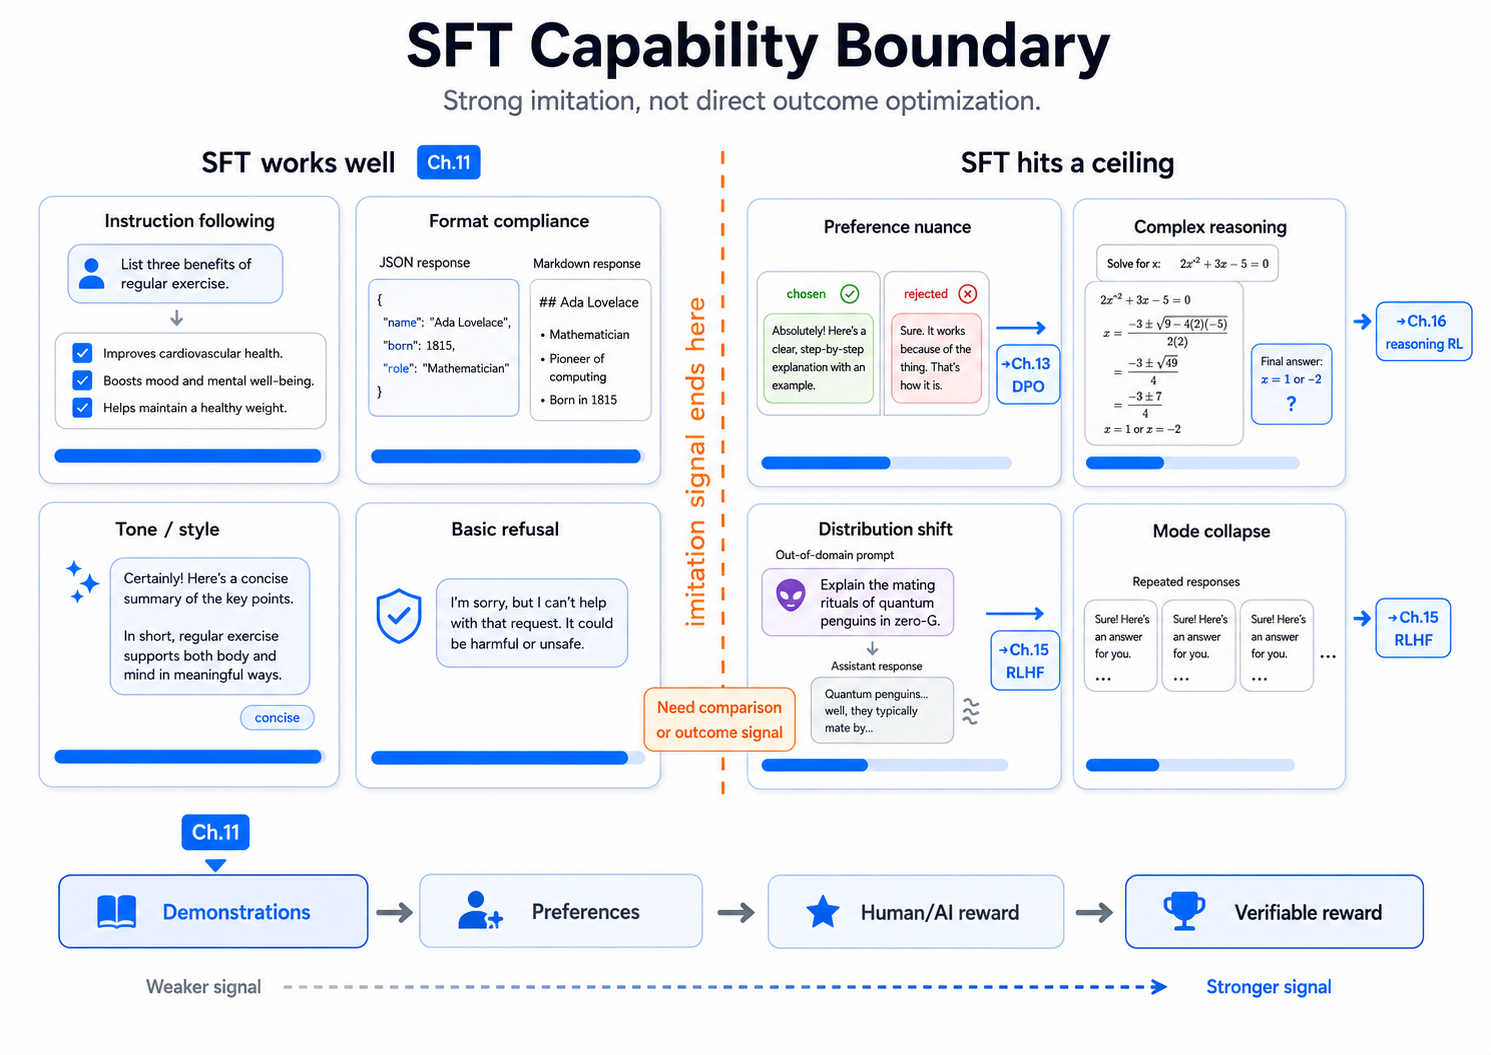
\includegraphics[width=0.92\textwidth]{figures/ch11/fig_sft_boundary.png}
\caption{\textbf{Where SFT helps and where it reaches its boundary.} Demonstration learning is strong for instruction following, formatting, tone, and basic refusal behavior. It is weaker when the target requires comparing alternatives, optimizing outcomes, or discovering reasoning strategies. Those gaps motivate preference learning, RLHF, and reasoning RL in later chapters.}
\label{fig:sft-boundary}
\end{figure}

\begin{tcolorbox}[colback=gray!8, colframe=gray!50]
\small
Chapter~\ref{ch:data-engineering} taught: ``data quality is a hidden scaling axis---one that can rival the effect of doubling model size.'' Chapter~11's echo: \textbf{instruction data quality is the primary lever in post-training---it rivals the effect of switching algorithms.} Both chapters share the same lesson: when the algorithm is commoditized (SGD for pretraining, masked cross-entropy for SFT), the data becomes the design surface. This is not a coincidence. It is the same principle operating at a different stage of the pipeline.
\end{tcolorbox}

\begin{quickrecap}
\textbf{Quick Recap.}
\begin{itemize}[nosep,leftmargin=1.5em]
  \item SFT excels at instruction following, format compliance, and knowledge retrieval.
  \item SFT struggles with preference nuance, complex reasoning, distribution shift, and mode collapse.
  \item SFT plus preference optimization is the modern open-model default; full RL is most useful for frontier alignment and reasoning domains with verifiable rewards.
\end{itemize}
\textit{Next: how does today's SFT relate to the 2022 InstructGPT recipe that started it all?}
\end{quickrecap}


%======================================================================
\section{Modern SFT Has Come a Long Way}
\label{sec:instructgpt-callout}

This chapter has taught instruction tuning as it is practiced in 2024--2025: curated data, masked cross-entropy, careful formatting. But the technique has a history, and that history shapes how the rest of Part~III is organized. The callout below introduces a thread that runs through three chapters.

\begin{tcolorbox}[colback=orange!5, colframe=orange!60, title=\textbf{The InstructGPT Thread --- Preview}]
InstructGPT~\cite{ouyang2022instructgpt} introduced the three-stage post-training recipe: SFT $\to$ reward modeling $\to$ RLHF. In that paper, SFT alone (Stage~1) improved instruction-following behavior but hurt some broad capabilities relative to the base GPT-3. The full three-stage pipeline was needed to get the preferred assistant behavior without paying as much capability cost.

\medskip
Today, the picture is different. Carefully curated SFT is often strong enough to serve as the foundation for open instruction models, especially when followed by DPO-style preference tuning (Chapter~\ref{ch:preference-learning}) rather than a full classical RLHF stack (Chapter~\ref{ch:rlhf}). What changed is the data: InstructGPT's Stage~1 used $\sim$13K demonstrations; Llama-3-Instruct reportedly used millions of curated instruction examples spanning code, math, multi-turn dialogue, and safety; Tulu~3 (2024) introduced a systematic multi-stage curation pipeline that filters, deduplicates, and reweights across dozens of data sources. The scale and engineering of the data, not the loss function, is what separates 2024 SFT from 2022 SFT.

\medskip
This chapter's content is therefore closer to a complete first-pass assistant-tuning recipe than to InstructGPT's first stage. RLHF and reasoning RL remain essential for frontier-scale alignment and for capabilities (like sustained reasoning) that supervised learning cannot easily produce---but they are no longer the first tool most open-model practitioners reach for.

\medskip
\emph{This callout box is the first of three InstructGPT touchpoints in Part~III. Chapter~\ref{ch:preference-learning} uses InstructGPT as the RLHF baseline that DPO simplifies. Chapter~\ref{ch:rlhf} treats InstructGPT as the main RLHF case study. By the end of Chapter~\ref{ch:rlhf}, you will have InstructGPT as a fully developed mental model---but understood as historical foundation, not current best practice.}
\end{tcolorbox}

\noindent The distance between InstructGPT's 13K-example SFT and today's carefully curated larger pipelines is not primarily algorithmic---it is a data engineering gap. That gap is this chapter's central claim.

\begin{takeaways}
\textbf{Key Takeaways}
\begin{itemize}[nosep]
  \item Instruction tuning transforms a base language model from a text completer into an instruction-following model by changing the training distribution, not the architecture.
  \item SFT uses the same causal next-token loss as pretraining, but masks the loss to assistant tokens only. The model learns to imitate the assistant, not the user.
  \item Chat templates are part of the training contract. Template mismatch between training and inference is a silent failure mode.
  \item Instruction data quality has four practical dimensions: clear instructions, high-quality responses, broad task diversity, and consistent formatting.
  \item Synthetic and distilled data make SFT scalable, but they inherit the teacher model's errors, style, blind spots, and licensing constraints.
  \item SFT is excellent for instruction following and format compliance; preference learning and RL become necessary when the signal is comparative, outcome-based, or hard to demonstrate directly.
\end{itemize}
\end{takeaways}


%----------------------------------------------------------------------
\section*{Summary}

\paragraph{What this chapter established.} Instruction tuning transforms a pretrained language model into an instruction-following assistant using a conceptually simple recipe: take (instruction, response) pairs, compute cross-entropy loss on response tokens only, and train for a few epochs with a low learning rate. The mechanics are familiar from pretraining; the transformation is in the data.

\paragraph{The data-as-algorithm lesson.} The most important takeaway from this chapter is not the SFT loss function---that is identical to pretraining. It is the realization that \emph{when the algorithm is commoditized, data becomes the algorithm.} Llama-3-Instruct and Mistral-Instruct use the same loss, the same optimizer, and nearly the same architecture. They differ in what they trained on. Chapter~\ref{ch:data-engineering} made this argument for pretraining; this chapter makes it again for post-training, where the effect is even more pronounced because the dataset is smaller and each example carries more weight.

\paragraph{Three questions, three answers.}

\begin{quote}
\textbf{What are you training?} The same loss as pretraining, masked to response tokens. Chat templates mark role boundaries. Packing and attention masking make training efficient.

\smallskip
\textbf{Where does the data come from?} Four sources---human-written, template-based, LLM-generated, distillation---each with different quality--cost--scale profiles. Modern practice mixes sources and prioritizes quality over scale.

\smallskip
\textbf{What are the limits?} SFT excels at instruction following and format compliance. It struggles with preference nuance, complex reasoning, and distribution shift. SFT plus preference optimization is the modern open-model default; full RL is most useful for frontier alignment and verifier-backed reasoning.
\end{quote}

\paragraph{One sentence.} Instruction tuning does not teach the model new knowledge---it teaches the model to use its pretrained knowledge in response to human directives, and the data you train on matters more than the algorithm.

\paragraph{What comes next.} Chapter~\ref{ch:peft} asks whether you need to update all parameters to achieve this transformation. Chapter~\ref{ch:preference-learning} moves beyond imitation to preference-based training. Together, they complete the no-RL portion of post-training.


%----------------------------------------------------------------------
\section*{Key Equations at a Glance}

\begin{center}
\begin{tabularx}{\textwidth}{@{}p{5cm}X@{}}
\toprule
\textbf{Quantity} & \textbf{Expression} \\
\midrule
Pretraining loss & $\mathcal{L}_{\text{pretrain}} = -\frac{1}{T}\sum_{t=1}^{T} \log p_\theta(x_t \mid x_{<t})$ \\[4pt]
SFT loss (masked) & $\mathcal{L}_{\text{SFT}} = -\frac{1}{\sum_t m_t}\sum_{t=1}^{T} m_t \cdot \log p_\theta(x_t \mid x_{<t})$ \\[4pt]
Loss mask & $m_t = 1$ if token $t$ is assistant; $m_t = 0$ otherwise \\[4pt]
Typical SFT learning rate & $\eta \approx 10^{-5}$--$2 \times 10^{-5}$ (10$\times$--100$\times$ below pretraining) \\
\bottomrule
\end{tabularx}
\end{center}


%----------------------------------------------------------------------
\section*{Key Readings}

\begin{enumerate}[nosep]
  \item \textbf{Ouyang et al., 2022.} ``Training Language Models to Follow Instructions with Human Feedback'' (InstructGPT). Introduced the three-stage recipe. Read for historical context---SFT as Stage~1 of a larger pipeline.
  \item \textbf{Wei et al., 2022.} ``Finetuned Language Models Are Zero-Shot Learners'' (FLAN). Demonstrated that instruction tuning via task templates produces strong zero-shot generalization.
  \item \textbf{Wang et al., 2023.} ``Self-Instruct: Aligning Language Models with Self-Generated Instructions.'' The pipeline that enabled Alpaca and democratized instruction tuning.
  \item \textbf{Zhou et al., 2023.} ``LIMA: Less Is More for Alignment.'' The provocative quality-over-quantity result. Read alongside Tulu for the full picture.
  \item \textbf{Ivison et al., 2023.} ``Camels in a Changing Environment: Exploring the Role of Instruction Data'' (Tulu). Systematic study of instruction data mixtures---the empirical backbone for this chapter's data recommendations.
  \item \textbf{Taori et al., 2023.} ``Stanford Alpaca: An Instruction-Following LLaMA Model.'' The \$600 instruction-tuning demonstration.
  \item \textbf{Gunasekar et al., 2023.} ``Textbooks Are All You Need'' (Phi-1). Showed that structured synthetic data can match much larger models---the case for distillation.
\end{enumerate}

\flushbottom
